\chapter{\IfLanguageName{dutch}{Stand van zaken}{State of the art}}%
\label{ch:stand-van-zaken}

Dit hoofdstuk biedt een uitgebreide literatuurstudie over de verschillende aspecten van Edge Computing en de rol van databases in Edge-omgevingen.
Het is bedoeld om een grondige analyse te geven van de huidige stand van zaken binnen het onderzoeksdomein.
De inhoud van dit hoofdstuk bouwt voort op de inleiding en heeft als doel de lezer volledig op de hoogte te brengen van recente ontwikkelingen, technologieën en benaderingen die relevant zijn voor dit onderwerp, zodat zij het verdere verloop van de bachelorproef kunnen begrijpen zonder verdere opzoekingen te moeten doen.

\section{Bronnen zoekmethode}
De bronnen voor deze literatuurstudie werden gevonden door middel van een systematische zoekmethode, waarbij gebruik werd gemaakt van verschillende zoekmachines en databases, waaronder Google Scholar, IEEE Xplore, Semantic Scholar en Elicit.
Als zoektermen gebruikten we "EdgeDB", "Database on Edge" en "Edge Computing" \autocite{Yang2019EdgeDBAE, Paparrizos2021VergeDBAD, Gyorodi2015comparative}.

\section{Database on Edge}
De verschuiving naar gedecentraliseerde Edge Computing is onmiskenbaar, zoals treffend beschreven in het artikel "Het jaar van de Edge - alweer? Voor ongeveer de 10e keer op rij..." \autocite{Dollinger2022}. Toch lijkt het tempo van deze overgang trager te verlopen dan we oorspronkelijk hadden verwacht.

We zien dat er dagelijks een enorme hoeveelheid data wordt gegenereerd door de toenemende hoeveelheid verbonden apparaten, die de wereldwijde bevolking overstijgt. Deze data-explosie benadrukt des te meer het belang van Edge Computing, vooral nu het zijn hoogtepunt bereikt in de Gartner Life Cycle-hype.

\begin{figure}[h]
    \centering
    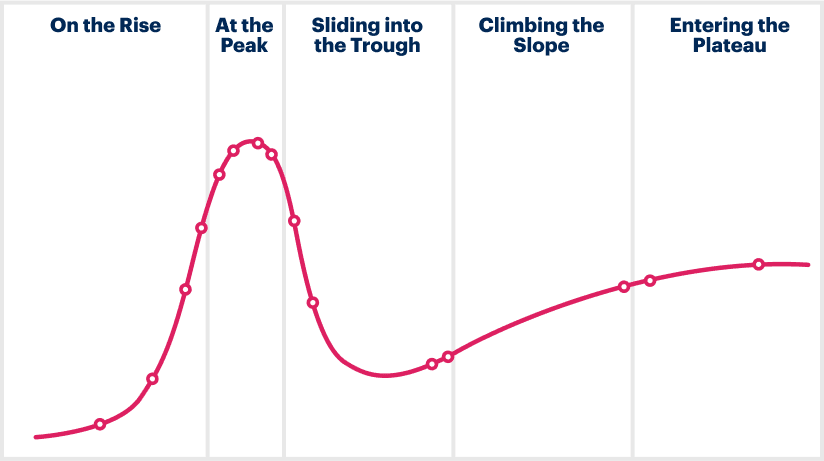
\includegraphics[width=0.5\textwidth]{hype-cycle-illustation.png}
    \caption{Gartner Hype Cycle, bron: \autocite{Gartner2023}}
    \label{fig:hype-cycle}
\end{figure}

Maar wat betekent die 'hypecyclus' eigenlijk? Wel, de Gartner Hype Cycle is eigenlijk een grafiek die laat zien hoe nieuwe technologieën populair worden en geaccepteerd raken. Het begint met veel opwinding, maar dan worden mensen vaak teleurgesteld als de technologie niet meteen alles waarmaakt wat ervan werd verwacht. Dan wordt de technologie realistisch bekeken en geleidelijk geaccepteerd, voordat ze uiteindelijk volwassen wordt en haar volledige potentieel bereikt.

Edge Computing gaat niet alleen over hardware, het gaat over hoe computers aan de rand van het netwerk werken. Het draait om systemen die verspreid zijn en niet centraal georganiseerd. Deze systemen zorgen voor uitdagingen, zoals het snel en betrouwbaar kunnen benaderen van gegevens in een verspreide omgeving.

Er zijn oplossingen voor deze uitdagingen, maar ze kosten vaak veel tijd en zijn lastig te schalen en te onderhouden. Bovendien is het moeilijk om geld te krijgen voor verbeteringen aan de infrastructuur, omdat mensen liever investeren in dingen die ze kunnen zien in plaats van in achterliggende verbeteringen.

De beperkingen van centrale cloudcomputing laten zien waarom Edge Computing zo belangrijk is. Door te werken aan de rand van het netwerk kunnen computers bijna in realtime reageren en ook zonder internetverbinding werken, terwijl de kosten voor het verzenden van gegevens naar centrale servers worden verlaagd.

Om de overgang naar Edge Computing makkelijker te maken, hebben we goede software nodig die werkt aan de rand van het netwerk. Edge Databases zijn hierbij cruciaal. Ze zorgen ervoor dat gegevens efficiënt kunnen worden opgeslagen en gedeeld tussen verschillende apparaten in een verspreide omgeving.

In tegenstelling tot traditionele software, passen Edge Databases goed in moderne technologiestacks en zorgen ze voor een efficiënter gebruik van middelen en snellere reactietijden. Dit helpt niet alleen de prestaties van apparaten te verbeteren, maar draagt ook bij aan milieuvriendelijker werken door het verminderen van CO2-uitstoot.

Kortom, Edge Databases zijn heel belangrijk voor de ontwikkeling van Edge Computing. Ze helpen bij het oplossen van de complexe problemen die komen kijken bij werken aan de rand van het netwerk en maken de weg vrij voor een bredere acceptatie van deze technologie.

\section{Databasearchitecturen}
In de wereld van databases is de architectuur de hoeksteen van hoe gegevens worden georganiseerd, opgeslagen en beheerd. Deze architectuur varieert afhankelijk van de specifieke behoeften en vereisten van een organisatie of applicatie. Laten we eens kijken naar enkele veelvoorkomende databasearchitecturen:

\section{EdgeDB: Een innovatieve tijdreeksdatabase voor Edge Computing}
EdgeDB is een innovatieve toevoeging op het gebied van tijdreeksdatabases, die een frisse benadering biedt voor het beheer van tijdreeksgegevens. Met nieuwe indexstructuren en geavanceerde queryverwerkingstechnieken belooft EdgeDB verbeterde prestaties en efficiëntie, waarbij het gebruik van TMTree een opvallend kenmerk is. Een grondige vergelijkende evaluatie van EdgeDB met gevestigde oplossingen zoals BTrDB en InfluxDB is noodzakelijk om inzicht te krijgen in de sterke punten en beperkingen ervan. Door evaluatiemetrics zoals invoegprestaties, schrijfprestaties, query-efficiëntie, geheugenoverhead en invoersnelheid van TMTree te analyseren, kunnen besluitvormers bepalen waar en hoe EdgeDB het beste kan worden ingezet binnen verschillende toepassingsdomeinen en gebruiksscenario's \autocite{Yang2019EdgeDBAE}.

\section{VergeDB: Een innovatieve tijdreeksdatabase voor Edge Computing}
Een recente ontwikkeling op het gebied van tijdreeksdatabases is VergeDB, een database die specifiek is ontworpen voor IoT-analytics op Edge-apparaten \autocite{Paparrizos2021VergeDBAD}. VergeDB belooft een innovatieve benadering te bieden voor het beheren van tijdreeksgegevens op de rand van het netwerk, wat cruciaal is voor real-time toepassingen waarbij snelle respons vereist is. Deze nieuwe database introduceert nieuwe compressiemethoden, indexstructuren en queryverwerkingstechnieken om de prestaties en efficiëntie te verbeteren. Een van de belangrijkste kenmerken van VergeDB is de mogelijkheid om gegevens lokaal op te slaan en te verwerken op Edge-apparaten, waardoor de latentie wordt verminderd en de prestaties worden verbeterd. VergeDB biedt ook ondersteuning voor geavanceerde analysetaken en machine learning-taken, zoals trendanalyse, patroonherkenning en anomaliedetectie, waardoor het een veelzijdige oplossing is voor diverse toepassingen op het gebied van IoT-analytics.

\section{Vergelijkende studie tussen MongoDB en MySQL}
Om een grondig begrip te krijgen van efficiënte oplossingen voor gegevensopslag in Edge Database-architecturen, is een vergelijkende studie uitgevoerd tussen MongoDB en MySQL. Deze vergelijking is van cruciaal belang om inzicht te krijgen in de verschillen tussen NoSQL (MongoDB) en relationele (MySQL) databases, met betrekking tot hun toepasbaarheid in Edge-omgevingen \autocite{Gyorodi2015comparative}.

\subsection{Databasekeuze voor Edge-omgevingen}

In Edge-omgevingen, waar latency en prestaties van vitaal belang zijn, speelt de keuze van de database een cruciale rol. MongoDB, als een NoSQL database, biedt flexibiliteit en schaalbaarheid, terwijl MySQL, als een relationele database, bekend staat om zijn gestructureerde en georganiseerde benadering van gegevensopslag. Het is essentieel om te begrijpen hoe deze verschillen zich vertalen naar de praktische implementatie in Edge-omgevingen \autocite{Gyorodi2015comparative}.

\subsection{Prestatievergelijking}

Een diepgaande analyse van de prestaties van MongoDB en MySQL in Edge-omgevingen is uitgevoerd. Hierbij zijn verschillende criteria geëvalueerd, waaronder:

\begin{itemize}
    \item Invoegoperaties: De snelheid en efficiëntie van het invoegen van gegevens in beide databases zijn vergeleken, rekening houdend met de vereisten voor real-time gegevensverwerking in Edge-omgevingen.
    \item Query-prestaties: Het vermogen van elke database om complexe queries uit te voeren en resultaten terug te geven binnen acceptabele latentietijden is beoordeeld, waarbij rekening wordt gehouden met de heterogeniteit van Edge-apparaten.
    \item Update- en verwijderingsoperaties: De snelheid en betrouwbaarheid van het bijwerken en verwijderen van gegevens in MongoDB en MySQL zijn geanalyseerd, met het oog op de dynamische aard van Edge-omgevingen.
\end{itemize}

\subsection{Gegevensintegriteit en consistentie}

Naast prestaties zijn ook gegevensintegriteit en consistentie van groot belang in Edge-omgevingen. MongoDB en MySQL bieden verschillende mechanismen voor het handhaven van gegevensintegriteit en consistentie, wat invloed heeft op de betrouwbaarheid van gegevens in dergelijke omgevingen \autocite{Gyorodi2015comparative}.

\subsection{Schalingsmogelijkheden}

Aangezien Edge-omgevingen vaak heterogeen en gedistribueerd zijn, is het onderzoeken van de schalingsmogelijkheden van MongoDB en MySQL van groot belang. Dit omvat het vermogen van elke database om te schalen met de groei van gegevens en de toename van het aantal Edge-apparaten, terwijl tegelijkertijd optimale prestaties worden gehandhaafd.

De resultaten van deze vergelijkende studie bieden inzicht in de meest geschikte databaseoplossing voor gegevensopslag in Edge Database-architecturen, waardoor de optimalisatie van gegevensopslag in Edge-omgevingen wordt verbeterd \autocite{Gyorodi2015comparative}.

\section{Vergelijkende studie tussen PostgreSQL, MongoDB en Neo4j}

Data vormt tegenwoordig een cruciale grondstof voor organisaties, omdat het hun manier van zakendoen, communiceren en besluitvorming heeft veranderd. Het fenomeen Big Data beschrijft een enorme hoeveelheid gestructureerde en ongestructureerde data, waarbij organisaties deze data analyseren om beslissingen te nemen en strategieën te ontwikkelen. Politieke partijen gebruiken bijvoorbeeld Big Data om de kans op verkiezingswinst van hun kandidaten te analyseren. In landen als Indonesië wordt Big Data echter nog niet optimaal benut vanwege beperkte infrastructuur. Daarom is het van essentieel belang dat Indonesië beschikt over een goede database die Big Data kan accommoderen \autocite{Gyorodi2015comparative}.

Eerdere onderzoeken hebben de prestaties van verschillende databases geanalyseerd, waaronder PostgreSQL, MongoDB en Neo4j. MongoDB bleek uitstekende prestaties te leveren met een complexiteit van O(1), terwijl PostgreSQL goede prestaties bood met complexiteiten van O(1) en O(n). Neo4j vertoonde echter een mindere prestatie met een complexiteit van O(n log n) \autocite{Gyorodi2015comparative}.

De studie omvatte het genereren van datasets, het modelleren van databases, het bouwen van databases, het implementeren van queries en het analyseren van de prestatietestresultaten. De datasets werden gegenereerd op basis van gegevens van de verkiezingsresultaten van 2019 voor de West-Javaanse verkiezingscommissie. De databases werden gemodelleerd en gebouwd voor PostgreSQL, MongoDB en Neo4j, elk met hun eigen database schema. Queries werden geïmplementeerd en uitgevoerd, en de prestatieresultaten werden geanalyseerd met behulp van Big O-notatie om de tijdcomplexiteit van elke database te meten \autocite{Gyorodi2015comparative}.

Query 1, die zocht naar vrouwelijke kiezers die op Partij A hebben gestemd, liet zien dat MongoDB uitstekende prestaties leverde met een complexiteit van O(1). PostgreSQL vertoonde goede prestaties met complexiteiten van O(1) en O(n), terwijl Neo4j een mindere prestatie leverde met een complexiteit van O(n log n). Voor Query 2, die zocht naar kiezers in het gebied Bogor die op Kandidaat A-3 hebben gestemd, vertoonden MongoDB en PostgreSQL vergelijkbare prestaties met complexiteit van O(1) en O(n), terwijl Neo4j weer een mindere prestatie leverde met een complexiteit van O(n log n).

Uit het onderzoek blijkt dat MongoDB uitstekende prestaties biedt als database voor het beheer van verkiezingsdata, met een complexiteit van O(1). PostgreSQL presteert ook goed, terwijl Neo4j de minste prestaties levert. Voor toekomstig onderzoek wordt aanbevolen om de prestaties van de databases te testen met betrekking tot het geheugengebruik \autocite{Gyorodi2015comparative}.


\section{Conclusie}
EdgeDB en VergeDB vertegenwoordigen innovatieve vooruitgangen in de wereld van tijdreeksdatabases voor Edge Computing. Beide databases bieden unieke voordelen op het gebied van prestaties, schaalbaarheid en efficiëntie, specifiek gericht op het beheren van tijdreeksgegevens in gedistribueerde omgevingen. EdgeDB maakt gebruik van geavanceerde indexstructuren en queryverwerkingstechnieken, wat resulteert in verbeterde invoeg- en schrijfprestaties. VergeDB introduceert nieuwe compressiemethoden en lokale opslagmogelijkheden, waardoor de latentie wordt verminderd en real-time analyse op Edge-apparaten mogelijk wordt.

Daarnaast toont de vergelijkende studie tussen MongoDB en MySQL de belangrijke verschillen tussen NoSQL en relationele databases in Edge-omgevingen. MongoDB biedt flexibiliteit en schaalbaarheid, terwijl MySQL bekend staat om zijn gestructureerde benadering van gegevensopslag. Beide benaderingen hebben hun eigen sterke punten en toepassingsgebieden, afhankelijk van de specifieke behoeften van de Edge-omgeving.

Het kiezen van de juiste databasearchitectuur is cruciaal voor het succes van Edge Computing-toepassingen. De keuze moet gebaseerd zijn op de specifieke eisen van de gegevensverwerking, schaalbaarheid en de dynamiek van de Edge-omgeving. Deze studie biedt een waardevolle gids voor het begrijpen van de huidige stand van zaken en het maken van geïnformeerde keuzes voor het beheren van tijdreeksgegevens aan de rand van het netwerk.